% Copyright 2006 by Till Tantau
%
% This file may be distributed and/or modified
%
% 1. under the LaTeX Project Public License and/or
% 2. under the GNU Free Documentation License.
%
% See the file doc/generic/pgf/licenses/LICENSE for more details.


A first example:

\begin{codeexample}[setup code,hidden]
    \usetikzlibrary{datavisualization}
\end{codeexample}
%
\begin{codeexample}[]
\begin{tikzpicture}[baseline]
  \datavisualization [
    school book axes,
    visualize as smooth line,
    clean ticks,
    all axes={grid={step=1,minor steps between steps=1}},
    x axis={
      ticks={
        major={
          also at={(0.5*pi) as $\pi/2$},
          also at={(pi) as $\pi$},
          options at=3 as [no tick text]
        }
      },
      label=$x$
    },
    y axis={
      label=$y$,
    }
  ]
  data [format=function] {
    var x : interval [-0.5*pi:4] samples 50;
    func y = sin(\value x r);
  };
\end{tikzpicture}
\end{codeexample}
\begin{codeexample}[preamble={\usetikzlibrary{datavisualization.formats.functions}}]
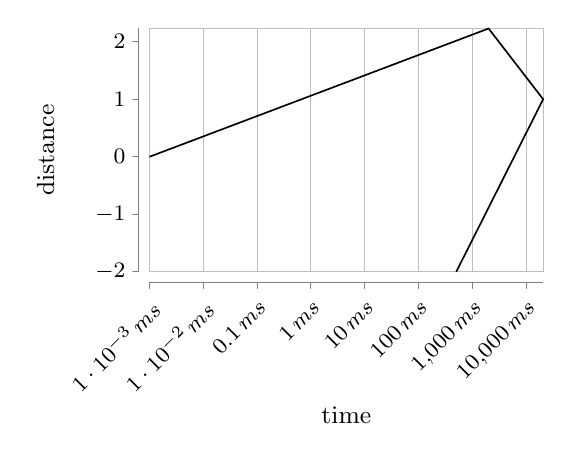
\begin{tikzpicture}[baseline]
  \datavisualization [
    scientific axes=clean,
    visualize as line,
    all axes={padding=4pt},
    x axis={logarithmic,
      ticks={many, tick unit={ms},
        node style={rotate=45,anchor=north east}},
      label={time},
      grid},
    y axis={label={distance}},
  ]
  data {
    x, y, z
    0.001, 0, 0
    2000, 2.23, 2
    20670, 1, 3
    501, -2, 0
  };
\end{tikzpicture}
\end{codeexample}

\begin{codeexample}[]
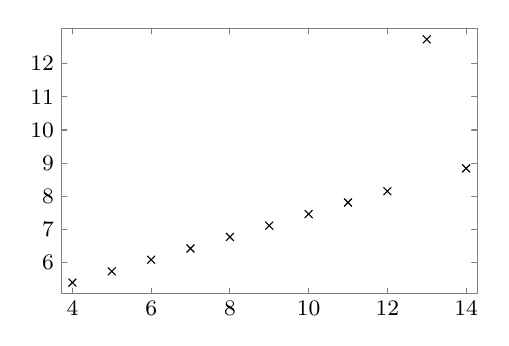
\begin{tikzpicture}[baseline,mark=*]
  \datavisualization [
    scientific axes=inner ticks,
    all axes={padding=4pt},
    euro about strategy,
    visualize as scatter,
    x axis={attribute=x2},
    y axis={attribute=y2}
  ]
  data [separator=\space] {
x       y       x1      y1      x2      y2      x3      y3
10.0    8.04    10.0    9.14    10.0    7.46    8.0     6.58
8.0     6.95    8.0     8.14    8.0     6.77    8.0     5.76
13.0    7.58    13.0    8.74    13.0    12.74   8.0     7.71
9.0     8.81    9.0     8.77    9.0     7.11    8.0     8.84
11.0    8.33    11.0    9.26    11.0    7.81    8.0     8.47
14.0    9.96    14.0    8.10    14.0    8.84    8.0     7.04
6.0     7.24    6.0     6.13    6.0     6.08    8.0     5.25
4.0     4.26    4.0     3.10    4.0     5.39    19.0    12.50
12.0    10.84   12.0    9.13    12.0    8.15    8.0     5.56
7.0     4.82    7.0     7.26    7.0     6.42    8.0     7.91
5.0     5.68    5.0     4.74    5.0     5.73    8.0     6.89
  };
\end{tikzpicture}
\end{codeexample}


%%% Local Variables:
%%% mode: latex
%%% TeX-master: "pgfmanual"
%%% End:
